% -*- Mode:TeX -*-

%% The documentclass options along with the pagestyle can be used to generate
%% a technical report, a draft copy, or a regular thesis.  You may need to
%% re-specify the pagestyle after you \include  cover.tex.  For more
%% information, see the first few lines of mitthesis.cls. 

%\documentclass[12pt,vi,twoside]{mitthesis}
%%
%%  If you want your thesis copyright to you instead of MIT, use the
%%  ``vi'' option, as above.
%%
%\documentclass[12pt,twoside,leftblank]{mitthesis}
%%
%% If you want blank pages before new chapters to be labelled ``This
%% Page Intentionally Left Blank'', use the ``leftblank'' option, as
%% above. 

\documentclass[12pt,twoside]{mitthesis}
\usepackage{lgrind}
\pagestyle{plain}

%% This bit allows you to either specify only the files which you wish to
%% process, or `all' to process all files which you \include.
%% Krishna Sethuraman (1990).

\typein [\files]{Enter file names to process, (chap1,chap2 ...), or `all' to
process all files:}
\def\all{all}
\ifx\files\all \typeout{Including all files.} \else \typeout{Including only \files.} \includeonly{\files} \fi

\begin{document}

% -*-latex-*-
% $Log: cover.tex,v $
% Revision 1.7  2001/02/08 18:53:16  boojum
% changed some \newpages to \cleardoublepages
%
% Revision 1.6  1999/10/21 14:49:31  boojum
% changed comment referring to documentstyle
%
% Revision 1.5  1999/10/21 14:39:04  boojum
% *** empty log message ***
%
% Revision 1.4  1997/04/18  17:54:10  othomas
% added page numbers on abstract and cover, and made 1 abstract
% page the default rather than 2.  (anne hunter tells me this
% is the new institute standard.)
%
% Revision 1.4  1997/04/18  17:54:10  othomas
% added page numbers on abstract and cover, and made 1 abstract
% page the default rather than 2.  (anne hunter tells me this
% is the new institute standard.)
%
% Revision 1.3  93/05/17  17:06:29  starflt
% Added acknowledgements section (suggested by tompalka)
% 
% Revision 1.2  92/04/22  13:13:13  epeisach
% Fixes for 1991 course 6 requirements
% Phrase "and to grant others the right to do so" has been added to 
% permission clause
% Second copy of abstract is not counted as separate pages so numbering works
% out
% 
% Revision 1.1  92/04/22  13:08:20  epeisach
\title{Probabilisitic Tractography and Its Applications in Neurological Studies}

\author{Tri M. Ngo}
\department{Department of Electrical Engineering and Computer Science}
% If the thesis is for two degrees simultaneously, list them both
% separated by \and like this:
% \degree{Doctor of Philosophy \and Master of Science}
\degree{Master of Engineering in Electrical Engineering and Computer Science}
\degreemonth{May}
\degreeyear{2007}
\thesisdate{May 28, 2007}

%% By default, the thesis will be copyrighted to MIT.  If you need to copyright
%% the thesis to yourself, just specify the `vi' documentclass option.  If for
%% some reason you want to exactly specify the copyright notice text, you can
%% use the \copyrightnoticetext command.  
%\copyrightnoticetext{\copyright IBM, 1990.  Do not open till Xmas.}

% If there is more than one supervisor, use the \supervisor command
% once for each.
\supervisor{Polina Golland}{Associate Professor}
\supervisor{Carl-Fredrik Westin}{Associate Professor}

% This is the department committee chairman, not the thesis committee
% chairman.  You should replace this with your Department's Committee
% Chairman.
\chairman{Arthur C. Smith}{Chairman, Department Committee on Graduate Students}

% Make the titlepage based on the above information.  If you need
% something special and can't use the standard form, you can specify
% the exact text of the titlepage yourself.  Put it in a titlepage
% environment and leave blank lines where you want vertical space.
% The spaces will be adjusted to fill the entire page.  The dotted
% lines for the signatures are made with the \signature command.
\maketitle

% The abstractpage environment sets up everything on the page except
% the text itself.  The title and other header material are put at the
% top of the page, and the supervisors are listed at the bottom.  A
% new page is begun both before and after.  Of course, an abstract may
% be more than one page itself.  If you need more control over the
% format of the page, you can use the abstract environment, which puts
% the word "Abstract" at the beginning and single spaces its text.

%% You can either \input (*not* \include) your abstract file, or you can put
%% the text of the abstract directly between the \begin{abstractpage} and
%% \end{abstractpage} commands.

% First copy: start a new page, and save the page number.
\cleardoublepage
% Uncomment the next line if you do NOT want a page number on your
% abstract and acknowledgments pages.
% \pagestyle{empty}
\setcounter{savepage}{\thepage}
\begin{abstractpage}
% $Log: abstract.tex,v $
% Revision 1.1  93/05/14  14:56:25  starflt
% Initial revision
% 
% Revision 1.1  90/05/04  10:41:01  lwvanels
% Initial revision
% 
%
%% The text of your abstract and nothing else (other than comments) goes here.
%% It will be single-spaced and the rest of the text that is supposed to go on
%% the abstract page will be generated by the abstractpage environment.  This
%% file should be \input (not \include 'd) from cover.tex.
Neuroscientists hypothesize that many neurological diseases are associated with neuroanatomical abnormalities.  Diffusion Tensor Imaging (DTI) allows us to probe and investigate anatomical differences in nerve fiber tracts. Current DTI clinical studies use voxel-based analysis.  Tractography is a better way to characterize fiber tracts.  Probabilistic tractography methods are even better because they provide a measure of uncertainty.  This project will enable novel studies fiber tract abnormalities by creating an interactive system for probabilistic tractography and an open-source implementation of the tractography algorithm. We will then use the system to study white matter structure and its changes in schizophrenia.

\end{abstractpage}

% Additional copy: start a new page, and reset the page number.  This way,
% the second copy of the abstract is not counted as separate pages.
% Uncomment the next 6 lines if you need two copies of the abstract
% page.
% \setcounter{page}{\thesavepage}
% \begin{abstractpage}
% % $Log: abstract.tex,v $
% Revision 1.1  93/05/14  14:56:25  starflt
% Initial revision
% 
% Revision 1.1  90/05/04  10:41:01  lwvanels
% Initial revision
% 
%
%% The text of your abstract and nothing else (other than comments) goes here.
%% It will be single-spaced and the rest of the text that is supposed to go on
%% the abstract page will be generated by the abstractpage environment.  This
%% file should be \input (not \include 'd) from cover.tex.
Neuroscientists hypothesize that many neurological diseases are associated with neuroanatomical abnormalities.  Diffusion Tensor Imaging (DTI) allows us to probe and investigate anatomical differences in nerve fiber tracts. Current DTI clinical studies use voxel-based analysis.  Tractography is a better way to characterize fiber tracts.  Probabilistic tractography methods are even better because they provide a measure of uncertainty.  This project will enable novel studies fiber tract abnormalities by creating an interactive system for probabilistic tractography and an open-source implementation of the tractography algorithm. We will then use the system to study white matter structure and its changes in schizophrenia.

% \end{abstractpage}

\cleardoublepage

\section*{Acknowledgments}

Thanks to lots of people.

%%%%%%%%%%%%%%%%%%%%%%%%%%%%%%%%%%%%%%%%%%%%%%%%%%%%%%%%%%%%%%%%%%%%%%
% -*-latex-*-

\pagestyle{plain}
  % -*- Mode:TeX -*-
%% This file simply contains the commands that actually generate the table of
%% contents and lists of figures and tables.  You can omit any or all of
%% these files by simply taking out the appropriate command.  For more
%% information on these files, see appendix C.3.3 of the LaTeX manual. 
\tableofcontents
\newpage
\listoffigures
\newpage
\listoftables


%% This is an example first chapter.  You should put chapter/appendix that you
%% write into a separate file, and add a line \include{yourfilename} to
%% main.tex, where `yourfilename.tex' is the name of the chapter/appendix file.
%% You can process specific files by typing their names in at the 
%% \files=
%% prompt when you run the file main.tex through LaTeX.
\chapter{Introduction}

\section{3D Slicer Interface}
\begin{figure}
	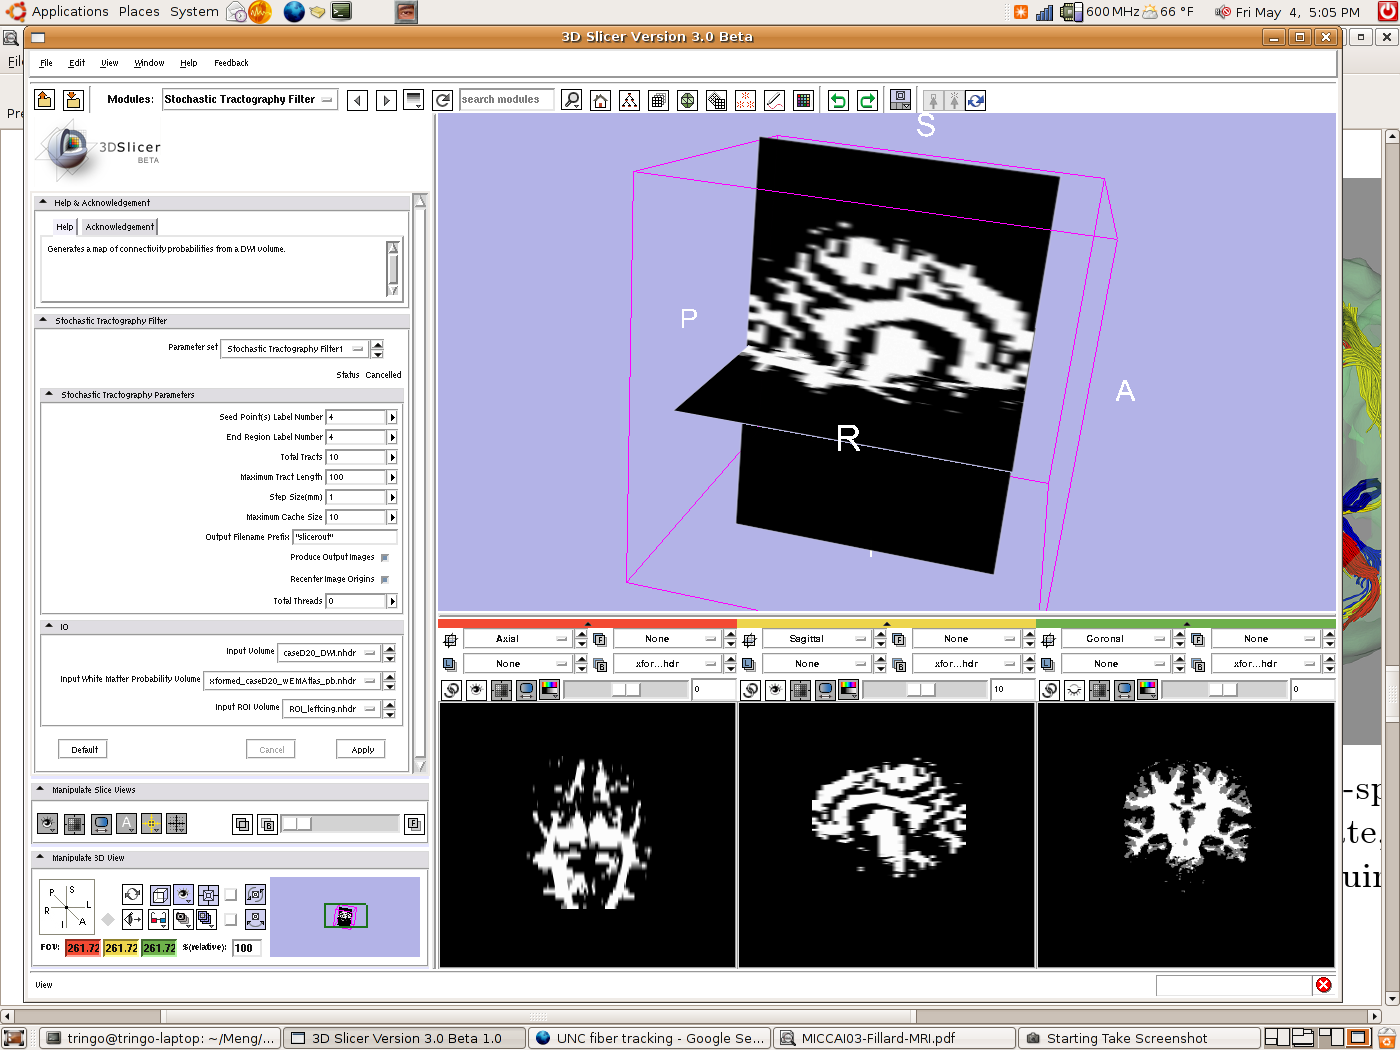
\includegraphics[width=0.5\linewidth]{slicermodule}
	\caption{Stochastic Tractography GUI module within 3D Slicer.}
	\label{fig:Intro}
\end{figure}

Magnetic Resonance Imaging (MRI) is a valuable imaging modality for studying the brain in-vivo.  We can use use MRI to differentiate between tissue types, which is useful in anatomical studies.  Diffusion Weighted Imaging (DWI) and more recently, Diffusion Tensor Imaging (DTI) provides a method to characterize white matter tracts, enabling studies of white matter architecture.

We can visualize DTI data sets using a number of methods.  DTI data sets provide information about the diffusion of water at each voxel, or volume element in the form of diffusion tensors.  A popular technique to visualize these diffusion tensors is to draw fiber tracts which utilize the diffusion information across many voxels.  This technique is known as DTI Tractography.

One possible method to perform tractography is to draw tracts which are oriented with the direction of maximal water diffusion of the voxels they pass through \cite{frimanTMI06}.  However, this method does not provide information about the uncertainty of the generated tracks due to noise or insufficient spatial resolution.  Stochastic white matter tractography addresses this problem by performing tractography under a probabilistic framework.  Stochastic methods provide additional information that enables clinical researchers to perform novel studies.  Several mathematical formulations of probabilistic tractography have existed for some time with the earliest being Behren's implementation\cite{behrensMRM03}.  However, tools which enable widespread adoption of stochastic tractography in clinical studies do not currently exist.  This research implements an easy to use system for performing stochastic white matter tractography based on the algorithm described by Friman et al. \cite{frimanTMI06}.

Researchers have hypothesized that white matter abnormalities may underlie some neurological conditions.  For instance, people characterize schizophrenia by its behavioral symptoms.  A short list of these these symptoms include auditory hallucinations, disordered thinking and delusion \cite{kubickiNYAS05}.  Studies have suggested that these behavioral symptoms have some connection with the neuroanatomical abnormalities observed in schizophrenia patients\cite{kubickiNYAS05}.  Researchers can noninvasively investigate the relationship between brain white matter abnormalities and schizophrenia by using white matter tractography.

Ultimately the success of the system developed in this thesis will depend on its use in the research community.  To this end, we implement the system within the open source ITK Segmentation and Registration Toolkit \cite{itk} framework.  ITK is currently used in many medical data processing applications.  ITK's large existing audience will encourage the system's use in the research community.  Additionally, implementing the stochastic tractography algorithm within ITK facilitates its integration into the 3D Slicer \cite{3Dslicer} for medical data visualization environment.  This thesis implements a 3D Slicer graphical user interface module for the stochastic tractography system, increasing its ease of use and further encouraging its application in clinical research (figure \ref{fig:Intro}).

Finally, we have applied this system towards the analysis of clinical schizophrenia DTI data.  Originally, the data was investigated using non-stochastic tractography methods.  We present a new investigation of the data using the system implemented in this research.  We also compare and contrast the results obtain from stochastic tractography and non-stochastic methods.

In this thesis we shall describe the motivation and implementation of the stochastic tractography system followed by a demonstration of possible applications of the system.  The next chapter  provides a background on nerve fiber tracts, DTI and prior work in white matter tractography.  After the background, the following chapter provides a detailed explanation of the stochastic tractography algorithm.  Then, we will describe the implementation of the algorithm within the ITK framework and optimizations used to improve performance.  Next, we demonstrate the system through an example analysis of frontal lobe nerve fiber bundles.  Finally, we will outline a clinical study which uses the algorithm to investigate differences in frontal lobe nerve fiber bundles in Schizophrenia.

\chapter{Background}


Diffusion Tensor Imaging (DTI or DTMRI) is a recently developed Magnetic Resonance (MR) technique that provides information about the diffusion of water molecules in throughout the brain.  In white matter, due to the interactions between water molecules and the surrounding nerve fibers, the principle diffusion direction is aligned with the local fiber orientation.

White matter tractography is a visualization and analysis tool for DTI data.  It takes local diffusion information provided by DTI images and produces estimates of fiber bundles which may explain the observed global diffusion distribution.  White matter tractography provides a means of characterizing fiber bundles in-vivo and may provide insights into questions concerning white matter architecture.

A number of clinical studies have used tractography to compare fiber bundle characteristics in different populations.  Many of these studies utilize tractography methods which do not provide a measure of the confidence regarding the estimated fiber bundles.  The stochastic tractography system implemented in this research provides these measures of confidence, and may open new avenues of clinical investigation of white matter architecture.

\section{Neuroanatomy and Fiber Tracts}
\begin{figure} \label{fig:fibertracts}
	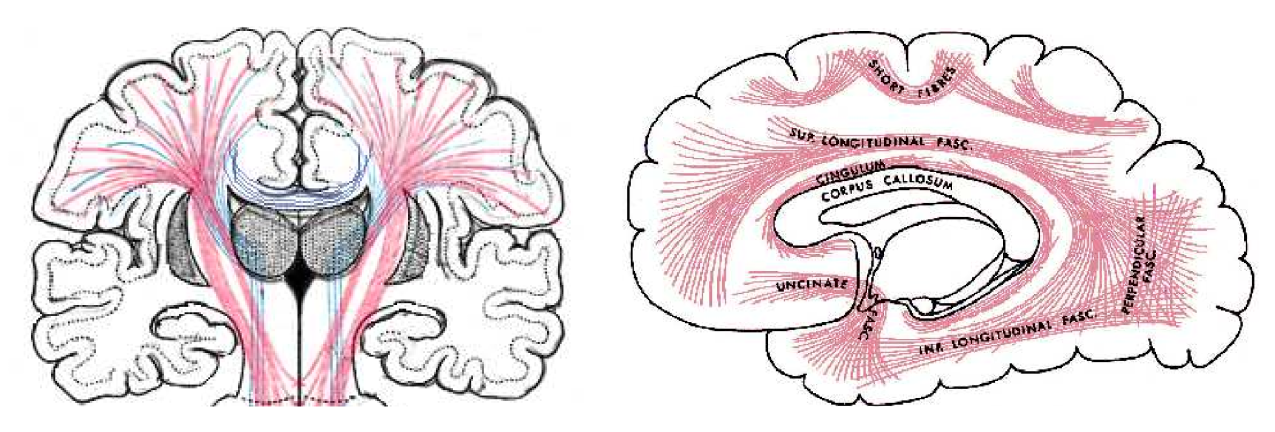
\includegraphics[width=\linewidth]{graysfibertracts}
	\caption{Example of human brain fiber tracts viewed from the front (coronal) and from the left (sagittal).  This image was derived from anatomical atlas diagrams in Gray's Anatomy \cite{odonnel06}.}
\end{figure}
Nerve tissue in the brain can be divided into gray and white matter.  Gray matter is found throughout the brain but is concentrated on the cortical surface as well as in structures deep within the brain such as the thalamus.  The defining characteristic of gray matter is its lack of myelinated axons.  In contrast white matter is white in color because it has an abundance of myelinated axons.  Myelin consists mostly of lipids and gives white matter its color.  Bundles of these axons comprise white matter tracts. Figure \ref{fig:fibertracts} illustrates some prominent fiber tracts.

\section{Diffusion Tensor MRI Physics}

Typically, MRI is used to differentiate between different tissue types, such as gray and white matter.  This technique works by magnetically polarizing a particular slice of the brain.  A strong uniform magnetic field is applied to the entire brain causing the spins of most of the electrons to orient in the same direction.  Another magnetic field, this one nonuniform in space, polarizes the spins of the atoms in the brain differently depending on their location.  This gradient field is turned off and as the spins of the electrons reorient, or relax, back to the strong uniform field, they release a radio signal which is picked up by the receiving coil.  The frequency of these waves depends on their polarization which is dependent on their position in space.  The time needed for the spins to relax, known as the relaxation time, depends on the type of tissue the molecules exist in.  Using this data, an image can be constructed that differentiates between tissue types due to their characteristic relaxation time. Unfortunately, white matter appears homogeneous in anatomical MRI images and do not provide much information about the orientation of the white fiber tracts within each voxel.  Without this information it is not possible to reliably determine the connectivity between different regions of gray matter.  Diffusion Tensor Imaging is a recently developed MR technique which provides more information to characterize fiber tracts.

Diffusion Tensor Imaging (DTI) or DTMRI is an imaging technique that indirectly provides information about fiber tract orientation from the diffusion profile of water in the brain tissues. Diffusion in many parts of the brain occurs anisotropically, meaning its rate of diffusion is directionally dependent.  This anisotropy is believed to be caused by local physical constraints that impede diffusion.  The diffusion of water molecules, which are the predominant signal emitters in MR imaging, is believed to be constrained by the myelin that surrounds axons.  DTI images describe the diffusion profile of water within each voxel using a diffusion tensor.  These tensors can be thought of as ellipsoids with the eigenvectors describing the major and minor axes of the ellipsoid and the associated eigenvalues scaling these axes.  Isotropic diffusion profiles result in spherical ellipsoids while anisotropic diffusion profiles produce more eccentric ellipsoids.  The parameters which describe these tensors are obtained from Diffusion Weighted Images (DWI) of the same volume captured using at least six unique gradient directions and one reference image obtained in the absence of weighting gradients.

Each Diffusion Weighted Image (DWI) provides information about the magnitude of diffusion in one particular direction.  Diffusion Weighted imaging works similarly to anatomical MRI imaging but is additionally able to capture the Brownian diffusion of molecules during the imaging process.  Unlike anatomical MRI, an additional gradient magnetic field is applied in a choosen direction which then makes the resulting observations sensitive to the self diffusion of water in that direction. An MRI image obtained using these diffusion sensitizing gradients is referred to as a Diffusion Weighted Image or DWI.  Associated with each of these images is the direction of the magnetic field gradient used to polarize the molecules.  This information is necessary because different magnetic field gradients may result in significantly different DWI images due to the anisotropy of diffusion in certain regions of the brain.  Finally, this diffusion information can be used to estimate the parameters of a diffusion tensor which is then used to infer the orientation of fiber tracts in that voxel.

\section{Diffusion Tensor}
The diffusion tensor is a 3x3 symetric matrix which describes the distribution of diffusion within each voxel.  Because the matrix is positive definite, its eigenvalues are positive and represent the magnetude of diffusion in the direction of the eigenvector associated with that eigenvalue.  The diffusion tensor is mostly represented as an ellipsoid, whose major and minor axis are described by the eigenvectors and associated eigenvalues of the tensor.  The eigenvector associated with the largest eigenvalue is sometimes referred to as the principle diffusion direction.  If the diffusion is sufficiently anisotropic, the principle diffusion direction is a good estimate of the local fiber orientation. %add physical meaning of the ellipsoid
%insert picture of ellipsoid

Because the tensor is sensitive to changes in the orientation of the object being scanned, clinical studies which attempt to compare different groups prefer to use properties of the tensor that are invariant to changes in orientation.  The most commonly used properties are the trace and the fractional anisotropy.  The trace the tensor is the sum of the diagonal components of the tensor and reprensents the average total diffusion.  A higher trace implies that there are few obstacles to water diffusion in that voxel.  The fraction anisotropy is given as
\begin{equation} \label{eq:tensormodel}
\sqrt{\frac{2*[(l\lambda_1-D_{av})^2 + (l\lambda_2-D_{av})^2 + (l\lambda_3-D_{av})^2]}
{2(\lambda_1^2+\lambda_2^2+\lambda_3^2)}}
\end{equation}

Fractional anisotropy is currently the most popular way to summarize the anisotropy of diffusion distribution expressed by the tensor.  FA ranges from 0 for isotropic diffusion to 1 for completely anisotropic diffusion.

%fill this in with related properties of the diffusion tensor
%various measures of anisotropy
%mathematic properties

\section{White Matter Tractography}

%[most have been voxel based,
% ROI studies, select a subset of voxels belonging to a particular fiber bundle of interest]
%[ROI studies sometimes select voxels in only one slice, which may not capture the information presented by the entire fiber tract...]


%[insert pictures]
%directionally coded images here
\begin{figure} \label{fig:visualization}
	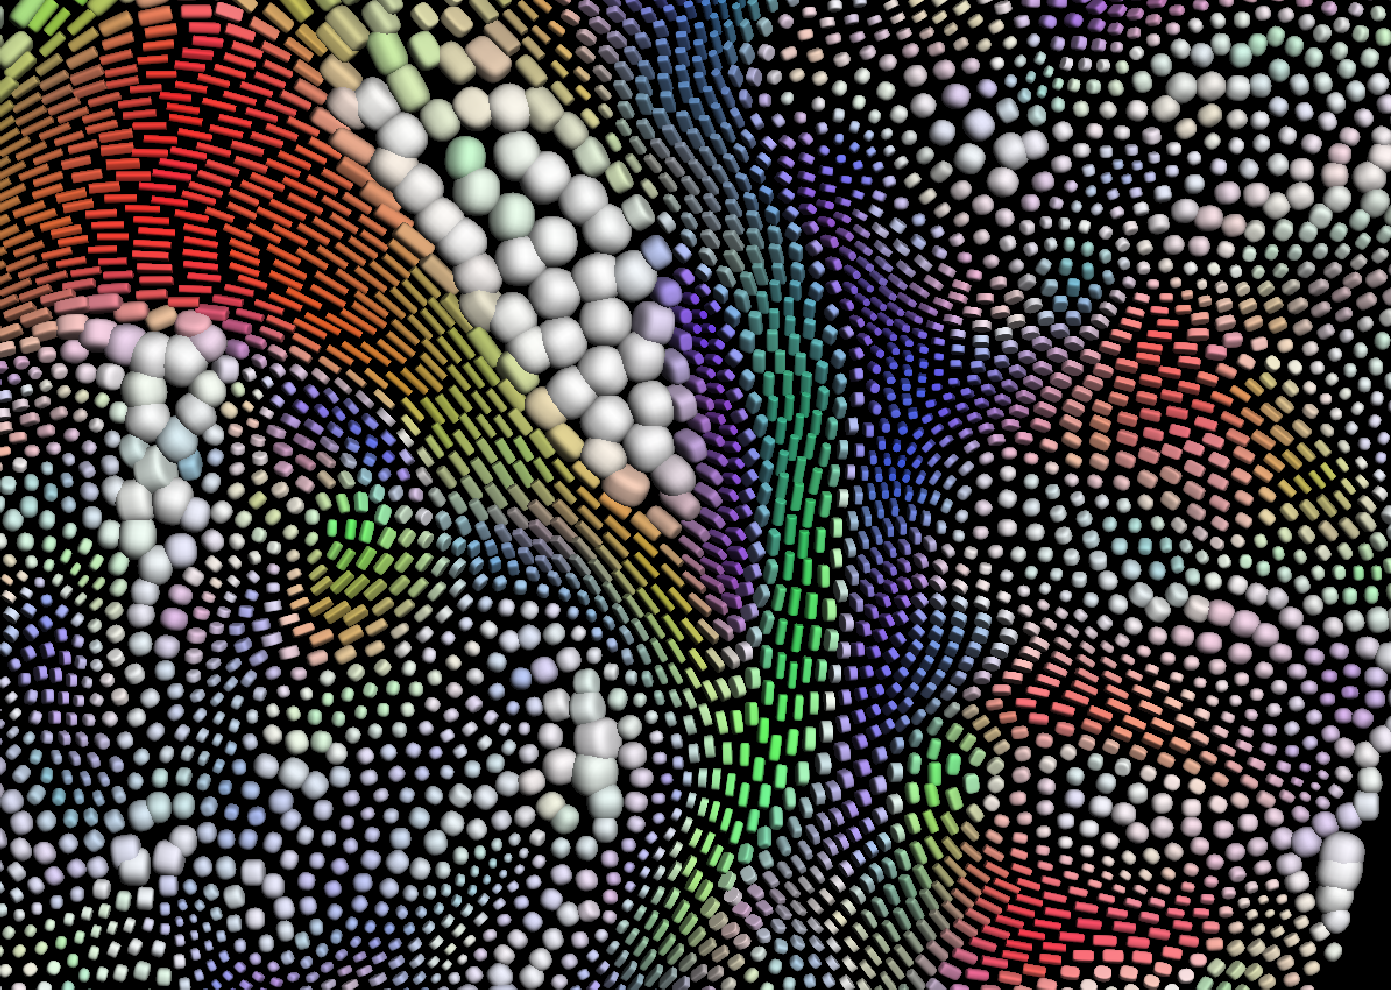
\includegraphics[width=0.5\linewidth]{packedglyphs}
	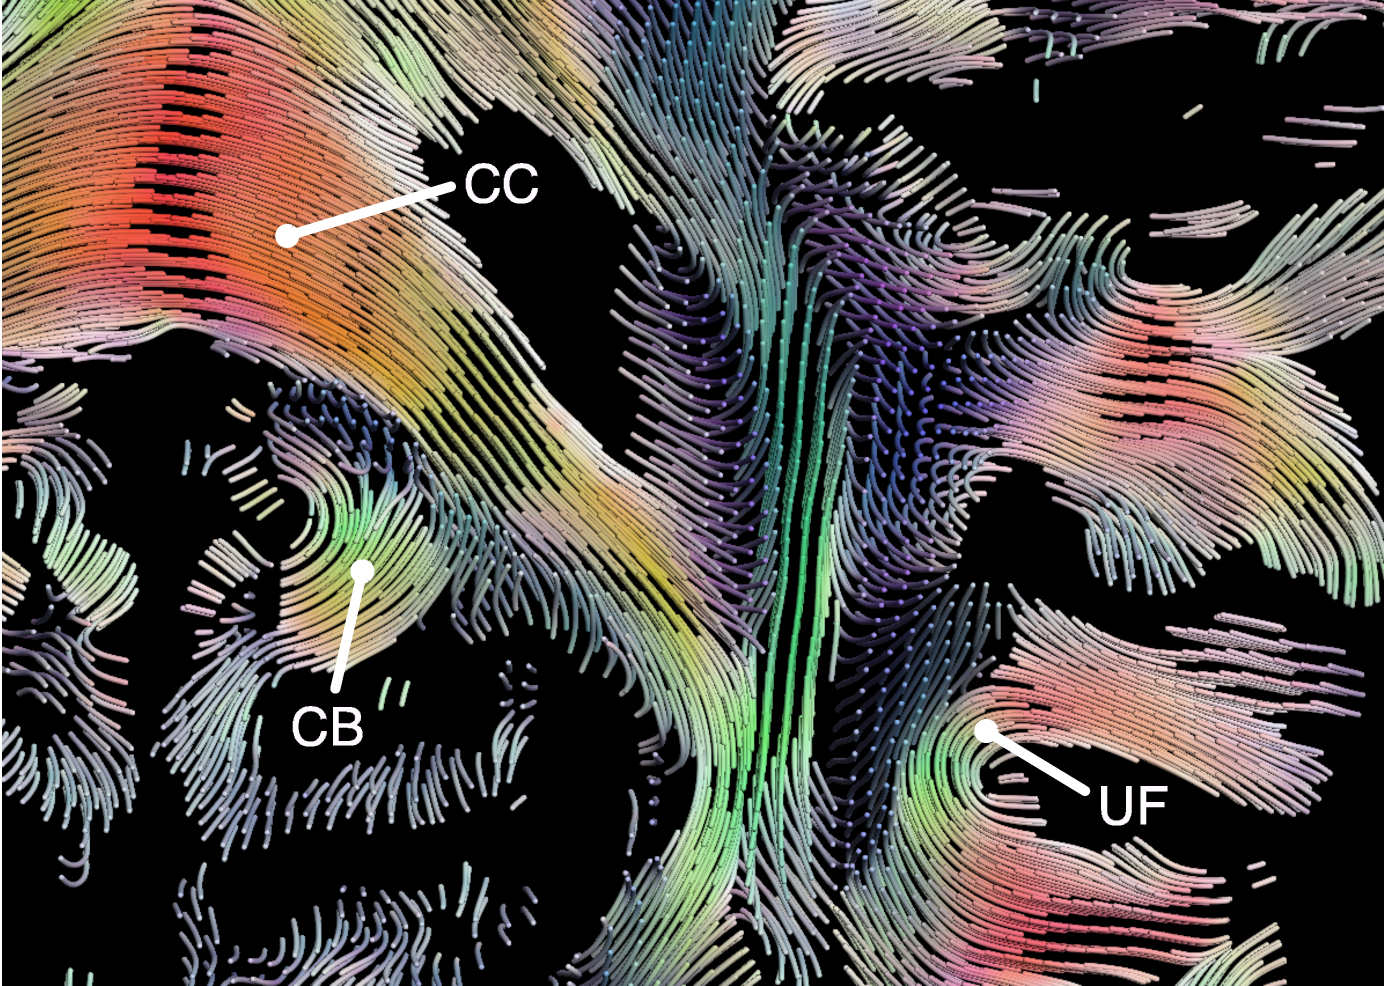
\includegraphics[width=0.5\linewidth]{tractography}
	\caption{DTI data visualization of major bundles using glyphs and streamlining tractography \cite{KindlmannTVCG2006}.  In the left image, DTI data is visualized using superquadric tensor glyphs. On the right, streamline tractography is performed on the same data.  The color in both images represent the estimated orientation of the fiber tract modulated by the degree of anisotropy in the data.  The color key is red is for left-right, blue for superior-inferior, green for anterior-posterior.  Regions that are white have low anisotropy while saturated regions exhibit highly anisotropic diffusion.}
\end{figure}


The two primary ways to visualize DTI data is through the use of glyphs and tractography.  Figure \ref{fig:visualization} demonstrates these two methods.  Glyphs are visual representations of the tensors at each voxel in one slice of DTI data.  The ellipsoid representation of the diffusion tensor can be also be used as a glyph but there exists many other representations that may provide a better visualization of the tensor field.  Glyph visualization is used for understanding diffusion in a localized region of interest.  Studies which compare local differences in DTI observations between different subjects are known as Region of Iterest or ROI studes. Although ROI analysis is straightforward, it is limited in the information it can provide and may actually introduce errors.  For instance, it is difficult to determine if observing a location along a fiber bundle in one patient corresponds to observing the same location in another patient.  Ultimately, clinical researchers are often interested in the global fiber bundles which produced these local DTI observations.  These fiber bundles span multiple voxels, limiting the usefulness of glyph visualization in holistic studies of fiber bundle characteristics.  These inquiries into the characteristics of fiber bundles led to the invention of white matter tractography.  In contrast with glyph visualization, white matter tractography incorporates diffusion information across multiple voxels in order to estimate a fiber bundle or bundles which could explain the observed diffusion data.

\subsection{Streamline Tractography Methods}
%talk about as many past works in DTI as possible
%name them by what the authors have called them
%Survey of White Matter Tractography
%Behrens
%Bootstrap
%Fast marching
%Stochastic Tractography

Tractography can be performed in a number of ways. One method is to draw tracts which are collinear with the principle direction of diffusion direction of every voxel it passes through.  These methods are collectively known as streamlining methods and have been suggested and characterized by a number of researchers \cite{behrensMRM03}.  Streamline tractography has relatively low computational cost and as such is very useful as a supplement to glyphs as a way to visualize DTI data.  However, streamline approaches do not provide information regarding the certainty of the estimated fiber tracts, limiting their usefulness in clinical studies which investigate white matter architecture characteristics.  Additionally, this lack of confidence information limits the regions that streamlining tractography can analyze.  Fiber orientation in regions which are highly isotropic are very uncertain.  Since streamlining methods do not account for this uncertainty, one cannot confidently analyze a region containing isotropic voxels using streamlining methods.  To reflect this limitation, many streamline methods will not estimate tracts which even momentarily pass through isotropic regions.  Unfortunately, isotropic voxels occur throughout the brain, even in regions with highly coherent fibers.  These voxels appear isotropic due to noise, distortions in the DTI data or due to limitations in imaging resolution which result in partial volume effects.  Partial volume effects are caused by fibers which cross within a single voxel.  Since these currently does not exist a widely accepted model to relate voxels containing multiple fiber orientations with the observed data, these crossings result in a diffusion distribution that is averaged amoung the crossing fiber, resulting in a diffusion distribution with reduced anisotropic.  Streamlining tractography's lack of robustness to isotropic diffusion limits its application in studies of fiber bundle characteristics.  These limitation motivated the invention of Stochastic or Probabilistic Tractography tractography algorithms.  This class of tractography algorithms overcomes the shortcomings of streamline methods by explicitly modeling the uncertainty in the local fiber orientation

\subsection{Stochastic Tractography Methods}
Stochastic tractography, sometimes known as probabilistic tractography, differs from streamlining methods in that it takes into account the uncertainty in fiber orientation when calculating estimates of fiber tracts.  Stochastic methods perform tractography under a probabilistic framework.  Under this framework, beliefs regarding the estimated local fiber orientation can be propagated to provide a measure of confidence regarding fiber tracts which span multiple voxels.  This explicit modeling and propagation of beliefs allows stochastic methods to generate tracts in regions of low anisotropy. Stochastic methods are able to generate tracts which momentarily pass through regions of low anisotropy because they integrate local fiber orientation uncertainty into the uncertainty of the entire tract.  The robustness of stochastic methods to local fiber orientation uncertainty has even enabled some studies to directly assess the connectivity of grey matter, which generally exhibits isotropic diffusion, with other regions of the brain\cite{behrensMRM03}.

\subsubsection{Bootstrap Method}

The Bootstrap Method is a stochastic method that calculates the degree of connectivity between different regions of the brain based on the variance in the original DTI data.  The obtains a measure of the variance of the DTI data by using redundant sets of DTI data and through the creation of new data which consist of recombinations of the original data.  In Jones et al. \cite{derek} research on the boot strap method, nine redundant sets of DWI volumes are obtained to perform the Bootstrap method.  Random combinations of portions of DWI volumes are sampled from this pool to generate a large number of complete mixed DWI sets known as bootstraps.  These complete mixed DWI sets are then converted to DTI images.  Standard streamline tractography is then performed on each bootstrap set at the same starting, or seed location.  A visitation percentage is then calculated for each voxel in the volume indicating the percentage of sample sets which generated a tract that passed through that particular voxel.  This visitation percentage can be interpreted as the probability that a voxel is connected to the seed point via a fiber tract.

\subsubsection{Bayesian Methods}
Stochastic tractography methods which use Bayesian frameworks express beliefs about estimated fiber tracts by generating a posterior probability distribution of fibers given the observed DTI data.   These tractography methods use a probabilistic model to relate the underlying fiber orientation with the observed DTI data.  The probabilistic model is applied to every voxel to generate a posterior distribution of possible fiber orientations given the observed diffusion in that voxel.  A streamline-like tractography method is then used to generate tracts by randomly sampling fiber directions from the fiber orientation posterior at each voxel as calculated by the local model.  The sampled tract is a realization of a random variable generated from the posterior distribution of fibers.  Since there are many possible paths, to obtain a good approximation of the posterior distribution of the, many paths must be sampled.  Additionally, similar to the Bootstrap method, the probability that region $A$ is connected to region $B$ can then be found by calculating the fraction of paths that pass through region $B$ originating from $A$.

Behrens's bayesian approach was one of the pioneering works in the field of stochastic tractography\cite{behrensMRM03}. An important idea in Behren's work is in keeping clear the distinction between estimating a general diffusion distribution from DWI data and estimating the local fiber orientation from DWI data.  Although an inference of the local fiber orientation can be made from the tensor model's principle diffusion direction, the tensor model is primarily a model to infer the distribution of diffusion given the data.  However, in stochastic tractography, we wish to infer the local fiber orientation from the observed diffusion data.  Behrens formulates this distinction by avoiding the tensor model altogether in favor of the two-compartment model. The two-compartment model makes the assumption that only a single fiber passes through a voxel.  Deviations from this simple model due to crossing fibers is captured as uncertainty in the fiber orientation.  In this model a voxel is described as two compartments whose net diffusion profile is the sum of a small anisotropic diffusion component that occurs in and around the fiber and a larger isotropic diffusion component outside of the fiber.\cite{behrensMRM03}.  The fiber orientation distribution is analytically intractable and Behrens overcomes this issue by computing the PDF using Markov Chain Monte Carlo (MCMC) techniques.  MCMC is a method to numerically integrate an analytically intractable integral.  

\appendix
\chapter{Mathematical Derivation}
%insert the theorem which finds the closest constrained model here
\section{Linearized Diffusion Tensor Model}
For each voxel in the DWI volume a signal intensity $z_i$ can be measured given a particular gradient strength $b_i$ and magnetic gradient direction $\mathbf{g}_{i}=(g_{ix} \quad g_{iy} \quad g_{iz})^T$.  The subscript $i$ enumerates multiple measurements of the same voxel under different magnetic gradient directions.

%insert tensor model reference below
The tensor model is a popular model used to describe the relationship between a particular gradient direction $\mathbf{g}_i$, the gradient strength in that direction $b_i$ and the measured voxel intensity $z_i$:  
%
%
\begin{equation} \label{eq:tensormodel}
z_{i}=z_0 e^{-b_i \mathbf{g}_i^T \mathbf{D} \mathbf{g}_i}
\end{equation}


\begin{equation} \label{eq:Dtensor}
\mathbf{D}=
\left( \begin{array}{ccc}
D_{xx} & D_{xy} & D_{xz} \\
D_{xy} & D_{yy} & D_{yz} \\
D_{xz} & D_{yz} & D_{zz} \\
\end{array} \right)
\end{equation}
%
%
where $\mathbf{D}$ is the diffusion tensor, encoded as a $3\times3$ matrix that describes the rate of diffusion in 3D space.  


Taking the log of both sides of the equation leads to a more tractable linear relationship:

\begin{equation} \label{eq:logtensormodel}
\log(z_i)=\log(z_0)-b_i \mathbf{g}_i^T \mathbf{D} \mathbf{g}_i
\end{equation}
%
%
The model is now in a linear form so that we can apply standard techniques such as least squares to estimate the diffusion parameters (the entries of the $\mathbf{D}$).  The linearized form can be further simplified by expanding the matrix multiplications and isolating the parameters into a separate vector.

\begin{equation} \label{eq:logtensormodelexpanded}
\log(z_i)=\mathbf{a}_i^T\mathbf{q}
\end{equation}

\begin{equation} \label{eq:xi}
\mathbf{a}_i=
\left( \begin{array}{ccccccc}
1 & -b_ig_{ix}^2 & -b_ig_{iy}^2 & -b_ig_{iz}^2 & -2b_ig_{ix}g_{iy} & -2b_ig_{ix}g_{iz} & -2b_ig_{iy}g_{iz}
\end{array} \right)^T
\end{equation}


\begin{equation} \label{eq:q}
\mathbf{q}=
\left( \begin{array}{ccccccc}
z_0 & D_{xx} & D_{yy} & D_{zz} & D_{xy} & D_{xz} & D_{yz}
\end{array} \right)^T
\end{equation}
%
%
The entries of the diffusion tensor $\mathbf{D}$ and the scaling factor $z_0$ now correspond to entries in the $\mathbf{q}$ vector.

There are 7 parameters that must be solved for in $\mathbf{q}$.  At least 6 additional independent equations are required in order to solve for the parameters.  These equations can be obtained by measuring the voxel intensity using at least 7 noncolinear gradient directions $g_i$ and optionally by varying the gradient strengths $b_i$.  However, more than 7 directions are required to estimate the variance of the original data, as we discuss later in this section. The full system of equations containing all $n$ measurements of a voxel can be succinctly represented in matrix form:
\begin{equation} \label{eq:fulllogtensor}
\log(\mathbf{z})=\mathbf{A}\mathbf{q}
\end{equation}
Where $\mathbf{A}$ is a $n\times7$ matrix and $\log(\mathbf{z})$ is an $n$ length vector of the $n$ voxel intensities.  The least squares solution has the following form:

%include the Gram-Schmidtt optimization
\begin{equation} \label{eq:LSUpsilon}
\hat{\mathbf{q}} = (\mathbf{A}^T\mathbf{A})^{-1}\mathbf{A}^T\log(\mathbf{z})
\end{equation}

\section{Constrained Diffusion Tensor Model}
Although the tensor model provides a good description of a general diffusion profile, ultimately we would like to estimate the distribution of the fiber orientations from the voxel intensities.  To simplify the tractography process we assume that each voxel contains only one fiber, and the majority of diffusion occurs in the single direction dictated by this single fiber.  The assumption is mathematically modeled by constraining the diffusion tensor to forcing the two smallest eigenvalues to be equal.  Under this constraint the eigen-decomposition of the diffusion tensor $\mathbf{D}$

\begin{equation} \label{eq:EigenD}
\mathbf{D} = \lambda_1 \mathbf{\hat{e_1}}\mathbf{\hat{e_1}}^T + 
\lambda_2 \mathbf{\hat{e_2}}\mathbf{\hat{e_2}}^T +
\lambda_3 \mathbf{\hat{e_3}}\mathbf{\hat{e_3}}^T
\end{equation}
%
%
is simplified by assuming the two smallest eigenvalues $\lambda_2 = \lambda_3 = \alpha $:

% a little confused about the expression below
\begin{eqnarray} \label{eq:ConstrainedEigenD}
\mathbf{D} & = & \lambda_1 \mathbf{\hat{e_1}}\mathbf{\hat{e_1}}^T +
\alpha (\mathbf{\hat{e_2}}\mathbf{\hat{e_2}}^T + \mathbf{\hat{e_3}}\mathbf{\hat{e_3}}^T) \nonumber\\
& = & (\lambda_1 - \alpha) \mathbf{\hat{e_1}}\mathbf{\hat{e_1}}^T + \alpha\mathbf{I} \nonumber\\
& = & \beta\mathbf{\hat{e_1}}\mathbf{\hat{e_1}}^T + \alpha\mathbf{I}
\end{eqnarray}
%
%
Substituting this expression into the tensor model in equation(\ref{eq:tensormodel}) yields the constrained model:

\begin{equation} \label{eq:ConstrainedModel}
z_{i} = z_0 e^{-\alpha b_i} e^{-\beta b_i (g_i^T\mathbf{\hat{v}} ) ^2}
\end{equation}
%
%
where $\mathbf{\hat{v}}$ represents $\mathbf{\hat{e_1}}$, the eigenvector associated with the largest eigenvalue.  This change emphasizes that the constrained model attempts to model the underlying fiber orientation and not the general diffusion profile.

The parameters of the constrained model can be derived from the parameters of the tensor model.  Given matrix $\mathbf{D}$ with the eigenvalue factorization of equation (\ref{eq:EigenD}), the closest symmetric matrix, in terms of the Frobenius norm \cite{frimanTMI06}, with the two equal smallest eigenvalues is:

\begin{equation} \label{eq:derivedmatrix}
\mathbf{S} = \lambda_1 \mathbf{\hat{e_1}}\mathbf{\hat{e_1}}^T + 
\frac{\lambda_2 + \lambda_3}{2} (\mathbf{\hat{e_2}}\mathbf{\hat{e_2}}^T +
\mathbf{\hat{e_3}}\mathbf{\hat{e_3}}^T)
\end{equation}
%
%
Hence after fitting the tensor model we obtain the constrained model parameters:

\begin{equation} \label{eq:constrainedparams}
\alpha = \frac{\lambda_2 + \lambda_3}{2},\;
\beta = \lambda_1 - \alpha,\;
\mathbf{\hat{v}} = \mathbf{\hat{e}}
\end{equation}

The additional constraints imposed by the constrained model reduces the goodness of fit, as compared to the diffusion tensor model, for voxels that do not exhibit anisotropic diffusion.  The reduction in anisotropy may be due to partial volume effects and the constrained model captures this uncertainty with an increase residual variance which translates into a wider fiber orientation likelihood function.

\section{Fiber Orientation Likelihood Function}

The log of the measured voxel intensity can be described as the log of the true intensity $z_i$ with some additive noise $\epsilon$:

\begin{equation} \label{eq:logsignal}
y_i = \log(z_i) + \epsilon_i
\end{equation}
%
%
For moderate levels of SNR, Salvador et al. \cite{salvador} demonstrates that the distribution of the noise (\ref{eq:logsignal}) is approximately normal with a mean of zero and a variance equal to the variance of the original complex data \cite{salvador}, divided by the square of the non-log noise-free voxel intensity:

\begin{equation} \label{eq:noisepdf}
p(\epsilon_i) = N \left( 0, \frac{\sigma_i^2}{z_i^2} \right)
\end{equation}
%
%
Therefore the resultant distribution of the log of the measured voxel intensity can be modeled by the same normal distribution, whose mean has been shifted by the log of the noise-free intensity:
\begin{equation} \label{eq:signalpdf}
p(y_i) = N\left( \log(z_i), \frac{\sigma_i^2}{z_i^2} \right)
\end{equation}
%
%
%An additional assumption must be made that the n measurements are independent, is this reasonable?
The joint distribution of the $n$ noisy voxel log-intensities is obtained by multiplying the $n$ distributions together.  It is assumed that the variance of the original complex data is constant across all $n$ measurements of a voxel.

\begin{equation} \label{eq:jointsignalpdf}
p(\mathbf{y}) = \prod_{i=1}^{n}N\left( \log(z_i), \frac{\sigma^2}{z_i^2} \right)
\end{equation}


In other words, equation (\ref{eq:jointsignalpdf}) is the likelihood of observing the measured data given the noise-free intensities $z_i$.  Since we cannot directly observe $z_i$ we estimate them by fitting parameters for the constrained model from the observed noisy data $\mathbf{y}$.  Hence, after substituting in the constrained model, $z_i$ becomes $\hat{z}_i$ and equation (\ref{eq:jointsignalpdf}) becomes the likelihood of observing the measured data given a choice of parameters for the constrained model.  Since the parameter of primary interest is the estimated fiber direction $\mathbf{\hat{v}}$, it is separated from the estimated secondary parameters $\mathbf{\hat{\theta}} = \{\hat{z}_0, \hat{\alpha}, \hat{\beta}, \hat{\sigma}^2\}$.  $\sigma^2$ is the variance of the original complex data \cite{salvador}, not the variance of the intensity $z_i$.  It can be estimated by calculating the residual variance after fitting the parameters of the constrained model.

%change this to use weighted least squares estimation
\begin{equation} \label{eq:ResVar}
\hat{\sigma}^2 = \frac{(\log(\mathbf{y})-\mathbf{A}\hat{\mathbf{q}})^T(\log(\mathbf{y})-\mathbf{A}\hat{\mathbf{q}})}{n - 7}
\end{equation}

\begin{equation} \label{eq:likelihood}
p(\mathbf{y}|\mathbf{\hat{v}},\mathbf{\hat{\theta}}) = \prod_{i=1}^{n}N\left( \log(\hat{z}_i), \frac{\hat{\sigma}^2}{\hat{z}_i^2} \right)
\end{equation}



\section{Connectivity Probability Function}
%To generate a fiber tract we must randomly select a fiber orientation probability density distribution 
%The distribution of primary interest is the the posterior distribution of the fiber orientation in a voxel given the data and the previous 
% given a choice for the parameters of the model ($\alpha, \beta, \mathbf{v}$)
% Voxels whose diffusion deviates significantly from the assumption that there exists only one primary direction of diffusion will exhibit a large residual variance.  This residual variance communicates information regarding the uncertainty of fiber orientation due to noise as well partial volume effects (crossing fibers).
 
A generated fiber tract $k$ of length $l$ can be modeled as string of $l$ unit vectors lined end to end: $\mathbf{v}_{k, 1:l} = \{\mathbf{\hat{v}}_1,\ldots,\mathbf{\hat{v}}_l\}_k$.  $\Omega_A^l$ is the set of all possible $l$ length paths that originate from point A.  A probability function can be defined on the path space for $l$ length paths: $p(\mathbf{v}_{k, 1:l})$ and consequently $p(\Omega_A^l)=1$.  Additionally, a discrete probability function $p(l)$ can be defined on the path length.
Given the diffusion measurements $\mathbf{y}$, the probability that region $A$ is connected to region $B$ by a fiber tract, assuming that the path length is independent of the diffusion measurements is:
\begin{equation} \label{eq:connectivity}
p(A\rightarrow B|\mathbf{y}) = \sum_{l=1}^{\infty} \int_{\Omega_{AB}^n}p(l)p(\mathbf{v}_{1:l}|\mathbf{y})
\end{equation}

In general, equations such as (\ref{eq:connectivity}) which contain multidimensional integrals over complex path spaces are not tractable analytically and must be calculated numerically.  The equations below provide a method to approximate equation (\ref{eq:connectivity}) numerically.  $N_l$ paths of length $l$ are sampled from the path space $\Omega_A^l$.  $\mathbb{I}$ is an indicator function that takes on the value 1 only if a particular $l$ length path $\mathbf{v}_{1:l}^k$ originating from region A passes through region B, and is 0 otherwise.  The indicator function is used to calculate the fraction of sampled paths originating in region A that pass through B, of a particular length $l$.  Finally, these fractions are weighted by the probability of the path length $p(l)$ and summed over all possible path lengths.  The infinite summation over path length converges because there is a maximum path length beyond which longer lengths have zero probability.

\begin{equation} \label{eq:indicator}
\mathbb{I} = \left\{ \begin{array}{ll}
	1 & \mathbf{v}_{k, 1:l} \in \Omega_{AB}^n \\
	0 & \textrm{otherwise}
	\end{array} \right.
\end{equation}

\begin{equation} \label{eq:numconnectivity}
p(A\rightarrow B|Y) \approx \sum_{l=1}^\infty \sum_{k=1}^{N_n} p(l) \frac{\mathbb{I}(\mathbf{v}_{k,1:l})}{N_n}
\end{equation}

\section{Stochastic Fiber Tract Generation}
According to equation (\ref{eq:numconnectivity}), we must randomly sample tracts originating from region $A$.  These tracts can be generated stochastically, in the sense that the tract can be generated from repeated samples from a probability distribution.  In this case we are drawing from the distribution of fiber orientations at a given point in space.  This prior distribution can be refined by incorporating likelihood information from the constrained model, as well as prior information regarding the regularity of the fiber tract, to generate a posterior fiber orientation distribution.

\begin{equation} \label{eq:posterior}
p({\mathbf{\hat{v}}_i, \theta | \mathbf{\hat{v}}_{i-1}, \mathbf{y}}) =
\frac {p(\mathbf{y}| \mathbf{\hat{v}}_{i-1}, \mathbf{\hat{v}}_i, \theta) p(\mathbf{\hat{v}}_i, \theta | \mathbf{\hat{v}}_{i-1})}
{p(\mathbf{y}|\mathbf{\hat{v}}_{i-1})}
\end{equation}

Assuming the secondary parameters $\theta$ at the current point are independent of the previous step direction and prior knowledge about the next step direction: $p(\mathbf{\hat{v}}_i, \theta | \mathbf{\hat{v}}_{i-1}) = p(\mathbf{\hat{v}}_i | \mathbf{\hat{v}}_{i-1})p(\theta)$ and assuming diffusion measurements at the current point don't depend on the previous step direction: $p(\mathbf{y}| \mathbf{\hat{v}}_{i-1}, \mathbf{\hat{v}}_i, \theta) = p(\mathbf{y}| \mathbf{\hat{v}}_i, \theta)$ and $p(\mathbf{y}|\mathbf{\hat{v}}_{i-1}) = p(\mathbf{y})$ equation (\ref{eq:posterior}) simplifies:
%
%
\begin{equation} \label{eq:posteriorsimp}
p({\mathbf{\hat{v}}_i, \theta | \mathbf{\hat{v}}_{i-1}, \mathbf{y}}) =
\frac {p(\mathbf{y}| \mathbf{\hat{v}}_i, \theta) p(\mathbf{\hat{v}}_i | \mathbf{\hat{v}}_{i-1}) p(\theta)}
{p(\mathbf{y})}
\end{equation}
%
%
The denominator $p(\mathbf{y})$ normalizes the posterior probability distribution, allowing it to integrate to 1, and can be written as the integral of the numerator.
%
%
\begin{equation} \label{eq:normalization}
p(\mathbf{y}) = \int_{\mathbf{\hat{v}}_i, \theta} p(\mathbf{y}| \mathbf{\hat{v}}_i, \theta) p(\mathbf{\hat{v}}_i | \mathbf{\hat{v}}_{i-1}) p(\theta)
\end{equation}
%
%
The likelihood function $p(\mathbf{y}| \mathbf{\hat{v}}_i, \theta)$ is given by equation \ref{eq:likelihood}.

The prior probability function $p(\mathbf{\hat{v}}_i | \mathbf{\hat{v}}_{i-1})$ is used to encode knowledge about the regularity of fiber tracts.  While data from invasive studies nerve fibers can be used to estimate this PDF, for the purposes of this implementation a simple distribution given by (\ref{eq:prior}) where $\gamma \ge 0$ and $\frac{1}{\zeta}$ is a normalization factor that allows the distribution to integrate to 1.  This particular distribution gives preference to paths which continue in the prior direction and gives zero probability to perpendicular turns.  The most important function of the prior is to prevent the fiber tract from backtracking on itself.  Without the prior, this may occur because the likelihood function is symmetric.

\begin{equation} \label{eq:prior}
p(\mathbf{\hat{v}}_i | \mathbf{\hat{v}}_{i-1}) = 
\frac{1}{\zeta} \left\{\begin{array}{ll}
	(\mathbf{\hat{v}}_i^T\mathbf{\hat{v}}_{i-1})^\gamma & \mathbf{\hat{v}}_i^T\mathbf{\hat{v}}_{i-1} \ge 0, \\
	0 & \mathbf{\hat{v}}_i^T\mathbf{\hat{v}}_{i-1} < 0,
 \end{array} \right.
\end{equation}

Since we want to obtain the posterior PDF for the fiber direction alone, we must marginalize the joint posterior distribution (\ref{eq:posteriorsimp}) by integrating over the secondary parameters $\theta$.  To simplify this integration, we remove uncertainty regarding the secondary parameters, $\theta$ by assuming an ML estimate.  These ML estimates were calculated by fitting the constrained model (\ref{eq:constrainedparams}).  Under this assumption equation (\ref{eq:normalization}) simplifies to an integration only over the fiber directions $\mathbf{\hat{v}}_i$.  To simplify drawing samples from the posterior distribution, the continuous PDF (\ref{eq:posteriorsimp}) can by approximated by a discrete PDF as long as the continuous PDF is sampled finely enough.  Friman et al. \cite{frimanTMI06} found empirically that 2,562 directions spread evenly over a unit sphere $S$ was sufficient.  Taking these simplifications into account, equation (\ref{eq:posteriorsimp}) becomes:

\begin{equation} \label{eq:posteriordiscrete}
p(\mathbf{\hat{v}}_i|\mathbf{\hat{v}}_{i-1}, \mathbf{y}) = 
\frac{p(\mathbf{y}| \mathbf{\hat{v}}_i, \theta) p(\mathbf{\hat{v}}_i | \mathbf{\hat{v}}_{i-1})}
{\sum_{\mathbf{\hat{v}} \in \mathbf{S}} p(\mathbf{y}| \mathbf{\hat{v}}_i, \theta) p(\mathbf{\hat{v}}_i | \mathbf{\hat{v}}_{i-1})}
\end{equation}

Finally, since the probabilistic tractography is performed in the continuous space while the diffusion data is discretized, a decision must be made about which voxel's diffusion information should be used in the calculation of the posterior PDF at the current point.  This algorithm chooses an probabilistic interpolation method suggested by Behrens et al. \cite{behrensMRM03} which randomly selects a voxel near the current tract generation point, with closer voxels having a higher probability of being selected.

\chapter{Command Line Module Interface}
Below is the automatically generated output of the command line module when running the StochasticTractographyFilter program with the \texttt{--help} option.

\begin{verbatim}
USAGE:

   StochasticTractographyFilter  [--processinformationaddress
                                 <std::string>] [--xml] [--echo] [-j <int>]
                                 [-r] [-i] [-o <std::string>] [-c <int>]
                                 [-s <int>] [-m <int>] [-t <int>] [-e
                                 <int>] [-l <int>] [--] [--version] [-h]
                                 <std::string> <std::string> <std::string>


Where:

   --processinformationaddress <std::string>
     Address of a structure to store process information (progress, abort,
     etc.). (default: 0)

   --xml
     Produce xml description of command line arguments (default: 0)

   --echo
     Echo the command line arguments (default: 0)

   -j <int>,  --totalthreads <int>
     Total number of threads to use.  Default value of zero sets number of
     threads to number of CPUs (default: 0)

   -r,  --recenteroriginswitch
     Ignore the origins of the ROI and WM mask and set it to be the same as
     the DWI image origin (default: 0)

   -i,  --outputimageswitch
     Output Tensor, FA maps and Connectivity Maps (default: 0)

   -o <std::string>,  --outputprefix <std::string>
     Prefix for the output files (default: "Output")

   -c <int>,  --maxlikelihoodcachesize <int>
     Maximum Size of Likelihood Cache (default: 100)

   -s <int>,  --stepsize <int>
     The length of each segment of the tract in mm (default: 1)

   -m <int>,  --maxtractlength <int>
     Maximum Length of Sample Tract (default: 100)

   -t <int>,  --totaltracts <int>
     Number of Sample Tracts (default: 100)

   -e <int>,  --endlabelnumber <int>
     Label Number to use as end region (default: 1)

   -l <int>,  --labelnumber <int>
     Label Number to use as seed points (default: 0)

   --,  --ignore_rest
     Ignores the rest of the labeled arguments following this flag.

   --version
     Displays version information and exits.

   -h,  --help
     Displays usage information and exits.

   <std::string>
     (required)  Input DWI volume to be filtered

   <std::string>
     (required)  Input Mask volume that provides the probability that the
     voxel is white matter

   <std::string>
     (required)  Input ROI volume used to seed algorithm


   Description: Generates a map of connectivity probabilities from a DWI
   volume.

   Author(s): Tri Ngo
\end{verbatim}

%% This defines the bibliography file (main.bib) and the bibliography style.
%% If you want to create a bibliography file by hand, change the contents of
%% this file to a `thebibliography' environment.  For more information 
%% see section 4.3 of the LaTeX manual.
\bibliography{main}
\bibliographystyle{plain}

\end{document}

